\documentclass[notes,slidesec,a4]{seminar}
\usepackage[spanish]{babel}
\usepackage[utf8]{inputenc}

\usepackage{t-gsyc-6}
\usepackage{fancybox}
\usepackage{graphics}
\usepackage{moreverb}
\usepackage{alltt}
\usepackage{html}
\usepackage{hthtml}
\usepackage{amsmath}
\usepackage[normalsize]{subfigure}
\usepackage{url}
\usepackage{listings}

\usepackage{eurosym}

\title{VisualHFSM 5: recent improvements in
programming robots with automata in JdeRobot}
\author{Samuel Rey and José M. Cañas}

\cop{Samuel Rey Escudero}
\address{samuel.rey.escudero@gmail.com 
		josemaria.plaza@gmail.com}

\begin{document}
\maketitle

%%--------------------------------------------------------------

%\begin{hslide}
%\slsect{VisualHFSM 5: recent improvements in programming robots with automata in JdeRobot}

%\begin{center}

%Samuel Rey (samuel.rey.escudero@gmail.com) \\
%José M. Cañas (josemaria.plaza@gmail.com)

%\begin{figure}
%	
\includegraphics[height=2cm]{template/peloto.png}
%\end{figure}
%\end{center}

%\end{hslide}

%%--------------------------------------------------------------

\begin{hslide}
\slsect{Objectives}

The main objective is achieve a more mature, useful and flexible version of VisualHFSM. 

\begin{itemize}
\item Improve the usability and functionality of the graphical editor.
\item Show a runtime GUI with the automata state.
\item Generate Python components.
\item Make visualHFSM compatible with the ArDrone.
\end{itemize}

\end{hslide}

%%--------------------------------------------------------------

\begin{hslide}
\slsect{Graphical Editor's Improvements}

\begin{minipage}[t]{0.5\textwidth}
\begin{center}
	\begin{itemize}
	\item Easier navigation between hierarchy levels.
	\item Function \texttt{shutDown()} for ending the execution.
	\item More flexibility for creating the ICE configuration file.
	\item Can be executed from any directory.
	%%%\item Corregidos fallos presentes en versiones anteriores.
	\end{itemize}
\end{center}
\end{minipage}
\begin{minipage}[t]{0.5\textwidth}
\begin{center}
	\begin{figure}
		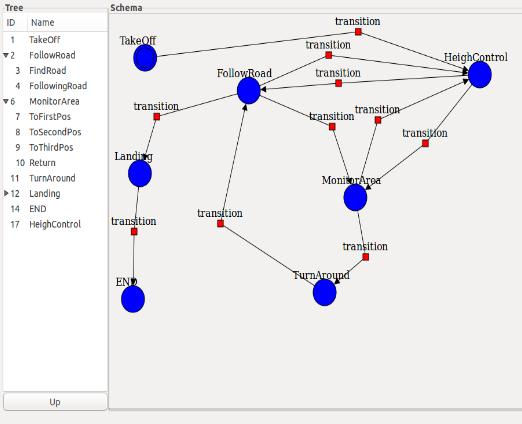
\includegraphics[height=3.5cm]{imgs/editor.png}
		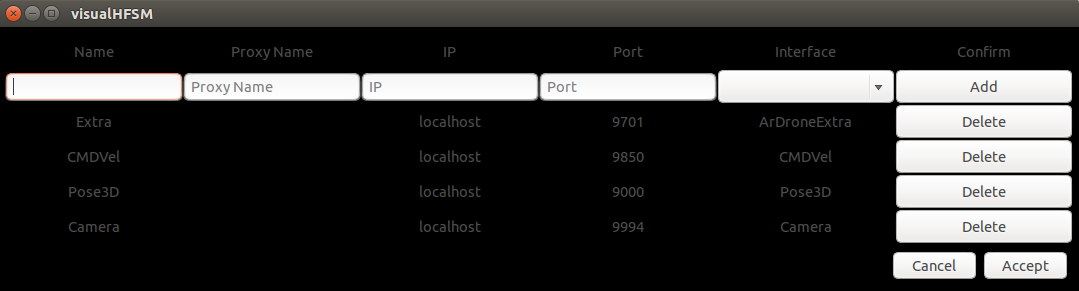
\includegraphics[height=1.5cm]{imgs/configFiles.png}
	\end{figure}
\end{center}
\end{minipage}

\end{hslide}

%%--------------------------------------------------------------

\begin{hslide}
\slsect{Runtime GUI in C++}

\begin{minipage}[t]{0.6\textwidth}
\begin{center}
	\begin{itemize}
	\item Shows dynamically the actives states in execution time.
	\item Similar appearance to the graphical editor.
	\item Deactivated by default. Can be activated with the argument \\
	 \textit{--displaygui=true}.
	\item Do not depend of the XML file.
	%\item Se utiliza un objeto \textit{Glib::Dispatcher} para notificar al hilo de la GUI cuando se ha producido un cambio en los estados.
	\item \textit{Autofocus} option.
	\end{itemize}
\end{center}
\end{minipage}
\begin{minipage}[t]{0.4\textwidth}
\begin{center}
	\begin{figure}
		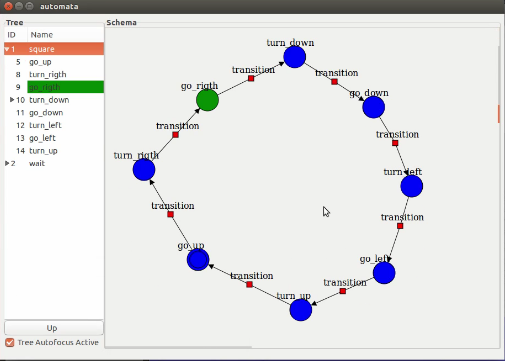
\includegraphics[height=4cm]{imgs/newRuntimeGuiCPP.png}
		%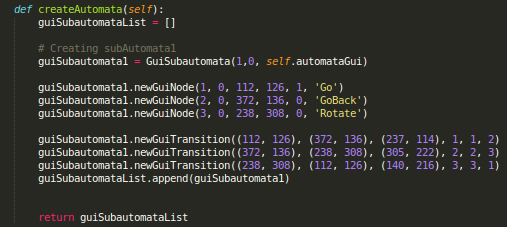
\includegraphics[height=2.5cm]{imgs/createAutomata.png}%Pasarla a transpa con plantilla??
	\end{figure}
\end{center}
\end{minipage}
\end{hslide}

%%--------------------------------------------------------------

\begin{hslide}
\slsect{Python components with runtime GUI}

\begin{itemize}
\item More flexibility for the tool.
\item Template organization a OOP model.
\item The runtime works like in the C++ components.
\item Allows visualizing more than one level at the same time.
\end{itemize}

\begin{center}
	\begin{figure}
		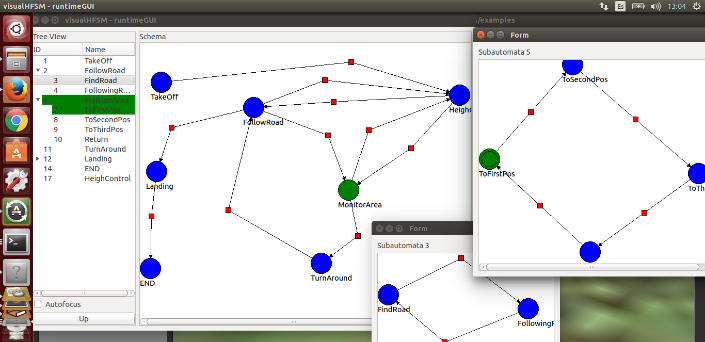
\includegraphics[height=3.5cm]{imgs/runtime-hierarchy.png}
	\end{figure}
\end{center}

\end{hslide}

%%--------------------------------------------------------------

%\begin{hslide}
%\slsect{Diffusion}

%Además de madurar y mejorar la funcionalidad de la herramienta, para que sea utilizada por terceros también nos hemos encargado de:
%\begin{itemize}
%\item Una documentación web, en el manual JdeRobot. 
%\item Escribir un artículo aceptado en el congreso robótico WAF 2016.
%\item Preparar un práctica Choca-Gira con en VisualHFSM dentro delentorno docente JdeRobot.
%\end{itemize}

%\end{hslide}

%%--------------------------------------------------------------

%\begin{hslide}
%\slsect{Experiments}

%This experiments shows:

%\begin{itemize}
%\item The news functionalities works properly.
%\item VisualHFSM is also compatible with drones.
%\end{itemize}

%3 Python applications:

%\begin{itemize}
%\item Bump \& Go.
%\item Monitor an Area.
%\item Follow the Colors with a drone.
%\end{itemize}

%\end{hslide}

%%--------------------------------------------------------------

\begin{hslide}
\slsect{Experiments}
\slsubsect{Bump \& Go}

\begin{itemize}
\item Simple application with a mono-level automata.
%\item Solución a la práctica propuesta en el entorno docente JdeRobot.
\end{itemize}

\begin{center}
\begin{minipage}[t]{0.45\textwidth}
	\begin{figure}
		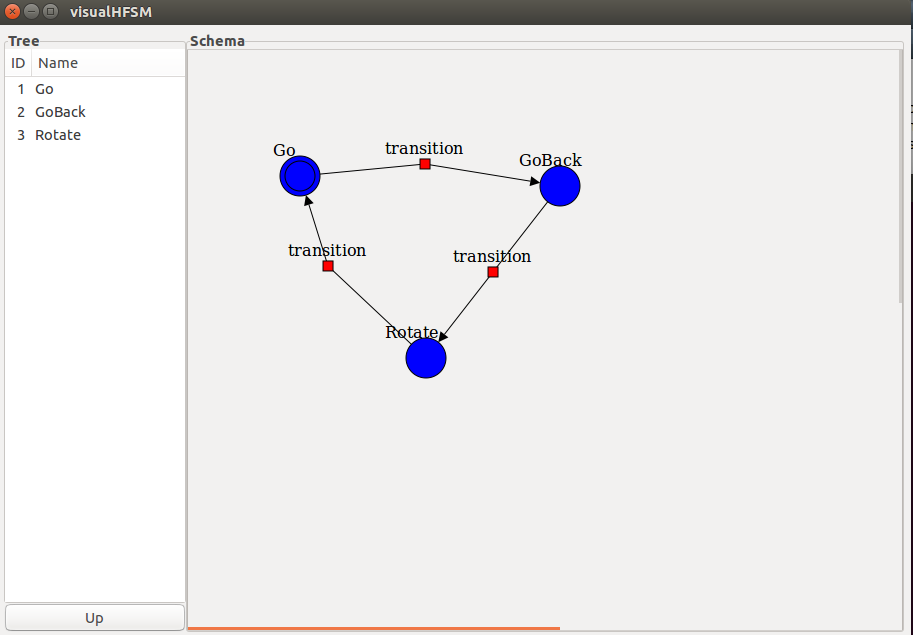
\includegraphics[height=3cm]{imgs/bumpAndGoDiagram.png}
	\end{figure}
\end{minipage}
\begin{minipage}[t]{0.45\textwidth}
	\begin{figure}
		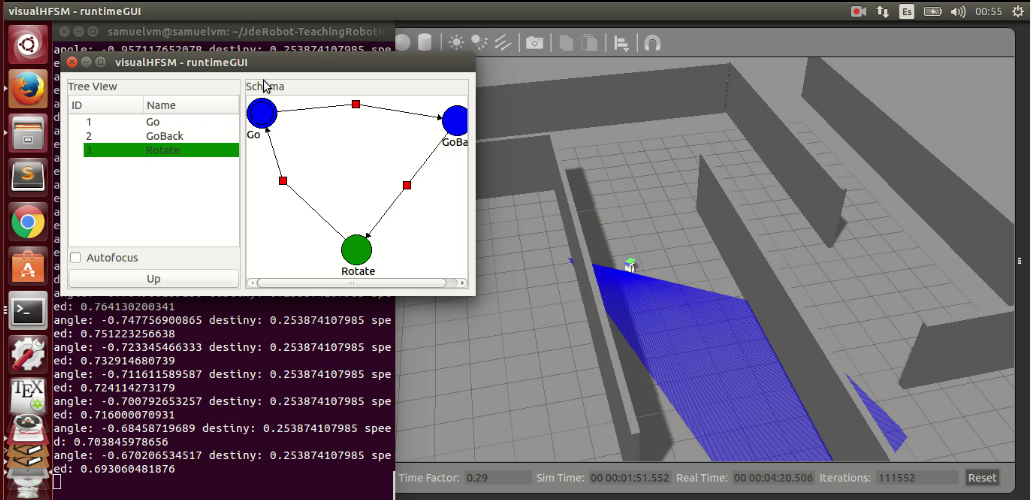
\includegraphics[height=3cm]{imgs/BAGRotate.png}
	\end{figure}
\end{minipage}
\end{center}

\end{hslide}


%%--------------------------------------------------------------

\begin{hslide}
\slsubsect{A drone monitors an area}

\begin{itemize}
\item More complex behaviour.
\item Multilevel automata.
\item Shows the compatibility with the ArDrone's interface in VisualHFSM.
\end{itemize}

\begin{center}
\begin{minipage}[t]{0.45\textwidth}
	\begin{figure}
		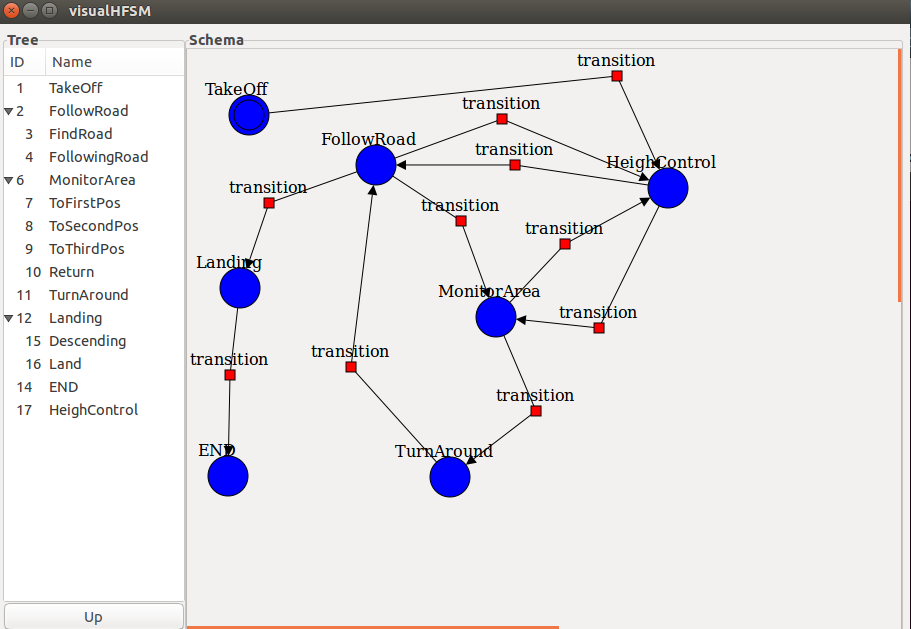
\includegraphics[height=3cm]{imgs/monitorArea.png}
	\end{figure}
\end{minipage}
\begin{minipage}[t]{0.45\textwidth}
	\begin{figure}
		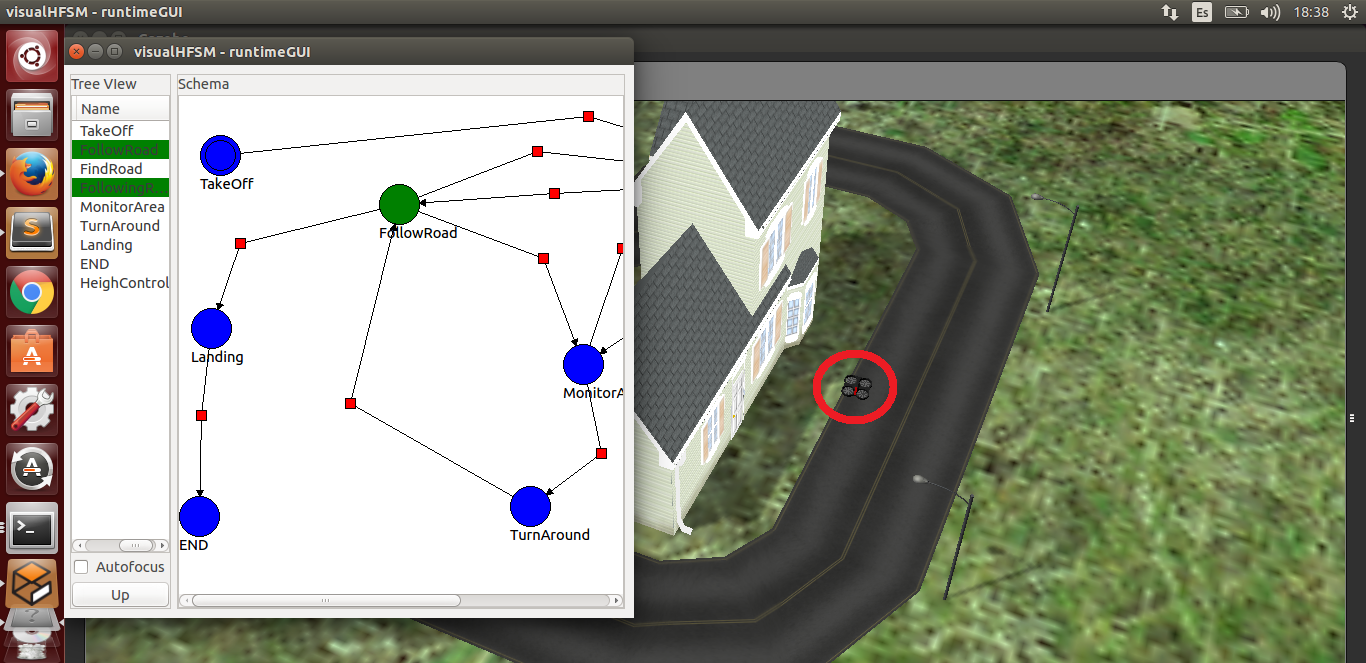
\includegraphics[height=3cm]{imgs/followingRoad.png}
	\end{figure}
\end{minipage}
\end{center}

\end{hslide}


%%--------------------------------------------------------------

\begin{hslide}
\slsubsect{A real drone follows the colors}

\begin{itemize}
\item Generated components are compatible with real robots.
\item Automata vs pure reactive systems.
\end{itemize}

\begin{center}
\begin{minipage}[t]{0.45\textwidth}
	\begin{figure}
		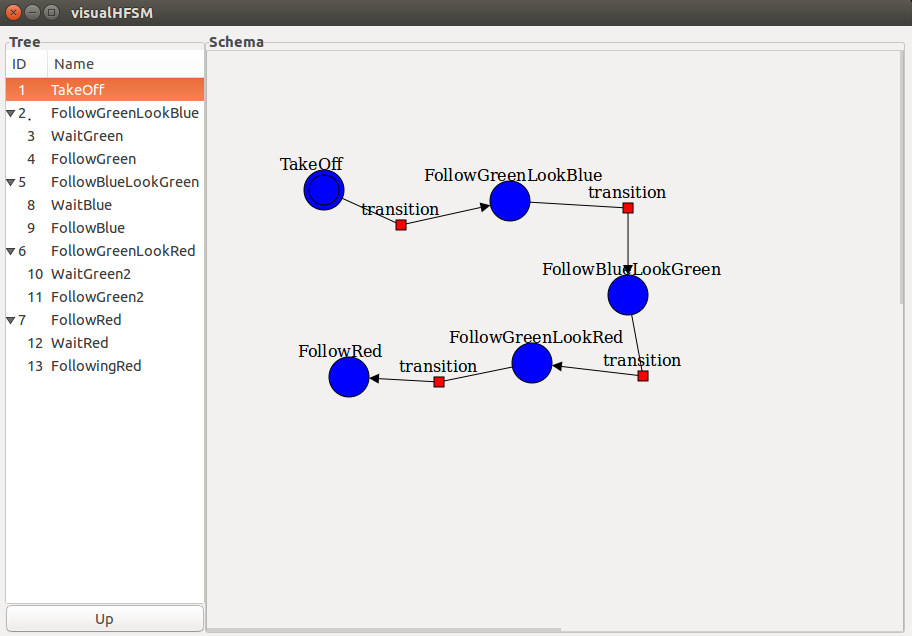
\includegraphics[height=3cm]{imgs/colorsDiagram.png}
	\end{figure}
\end{minipage}
\begin{minipage}[t]{0.45\textwidth}
	\begin{figure}
		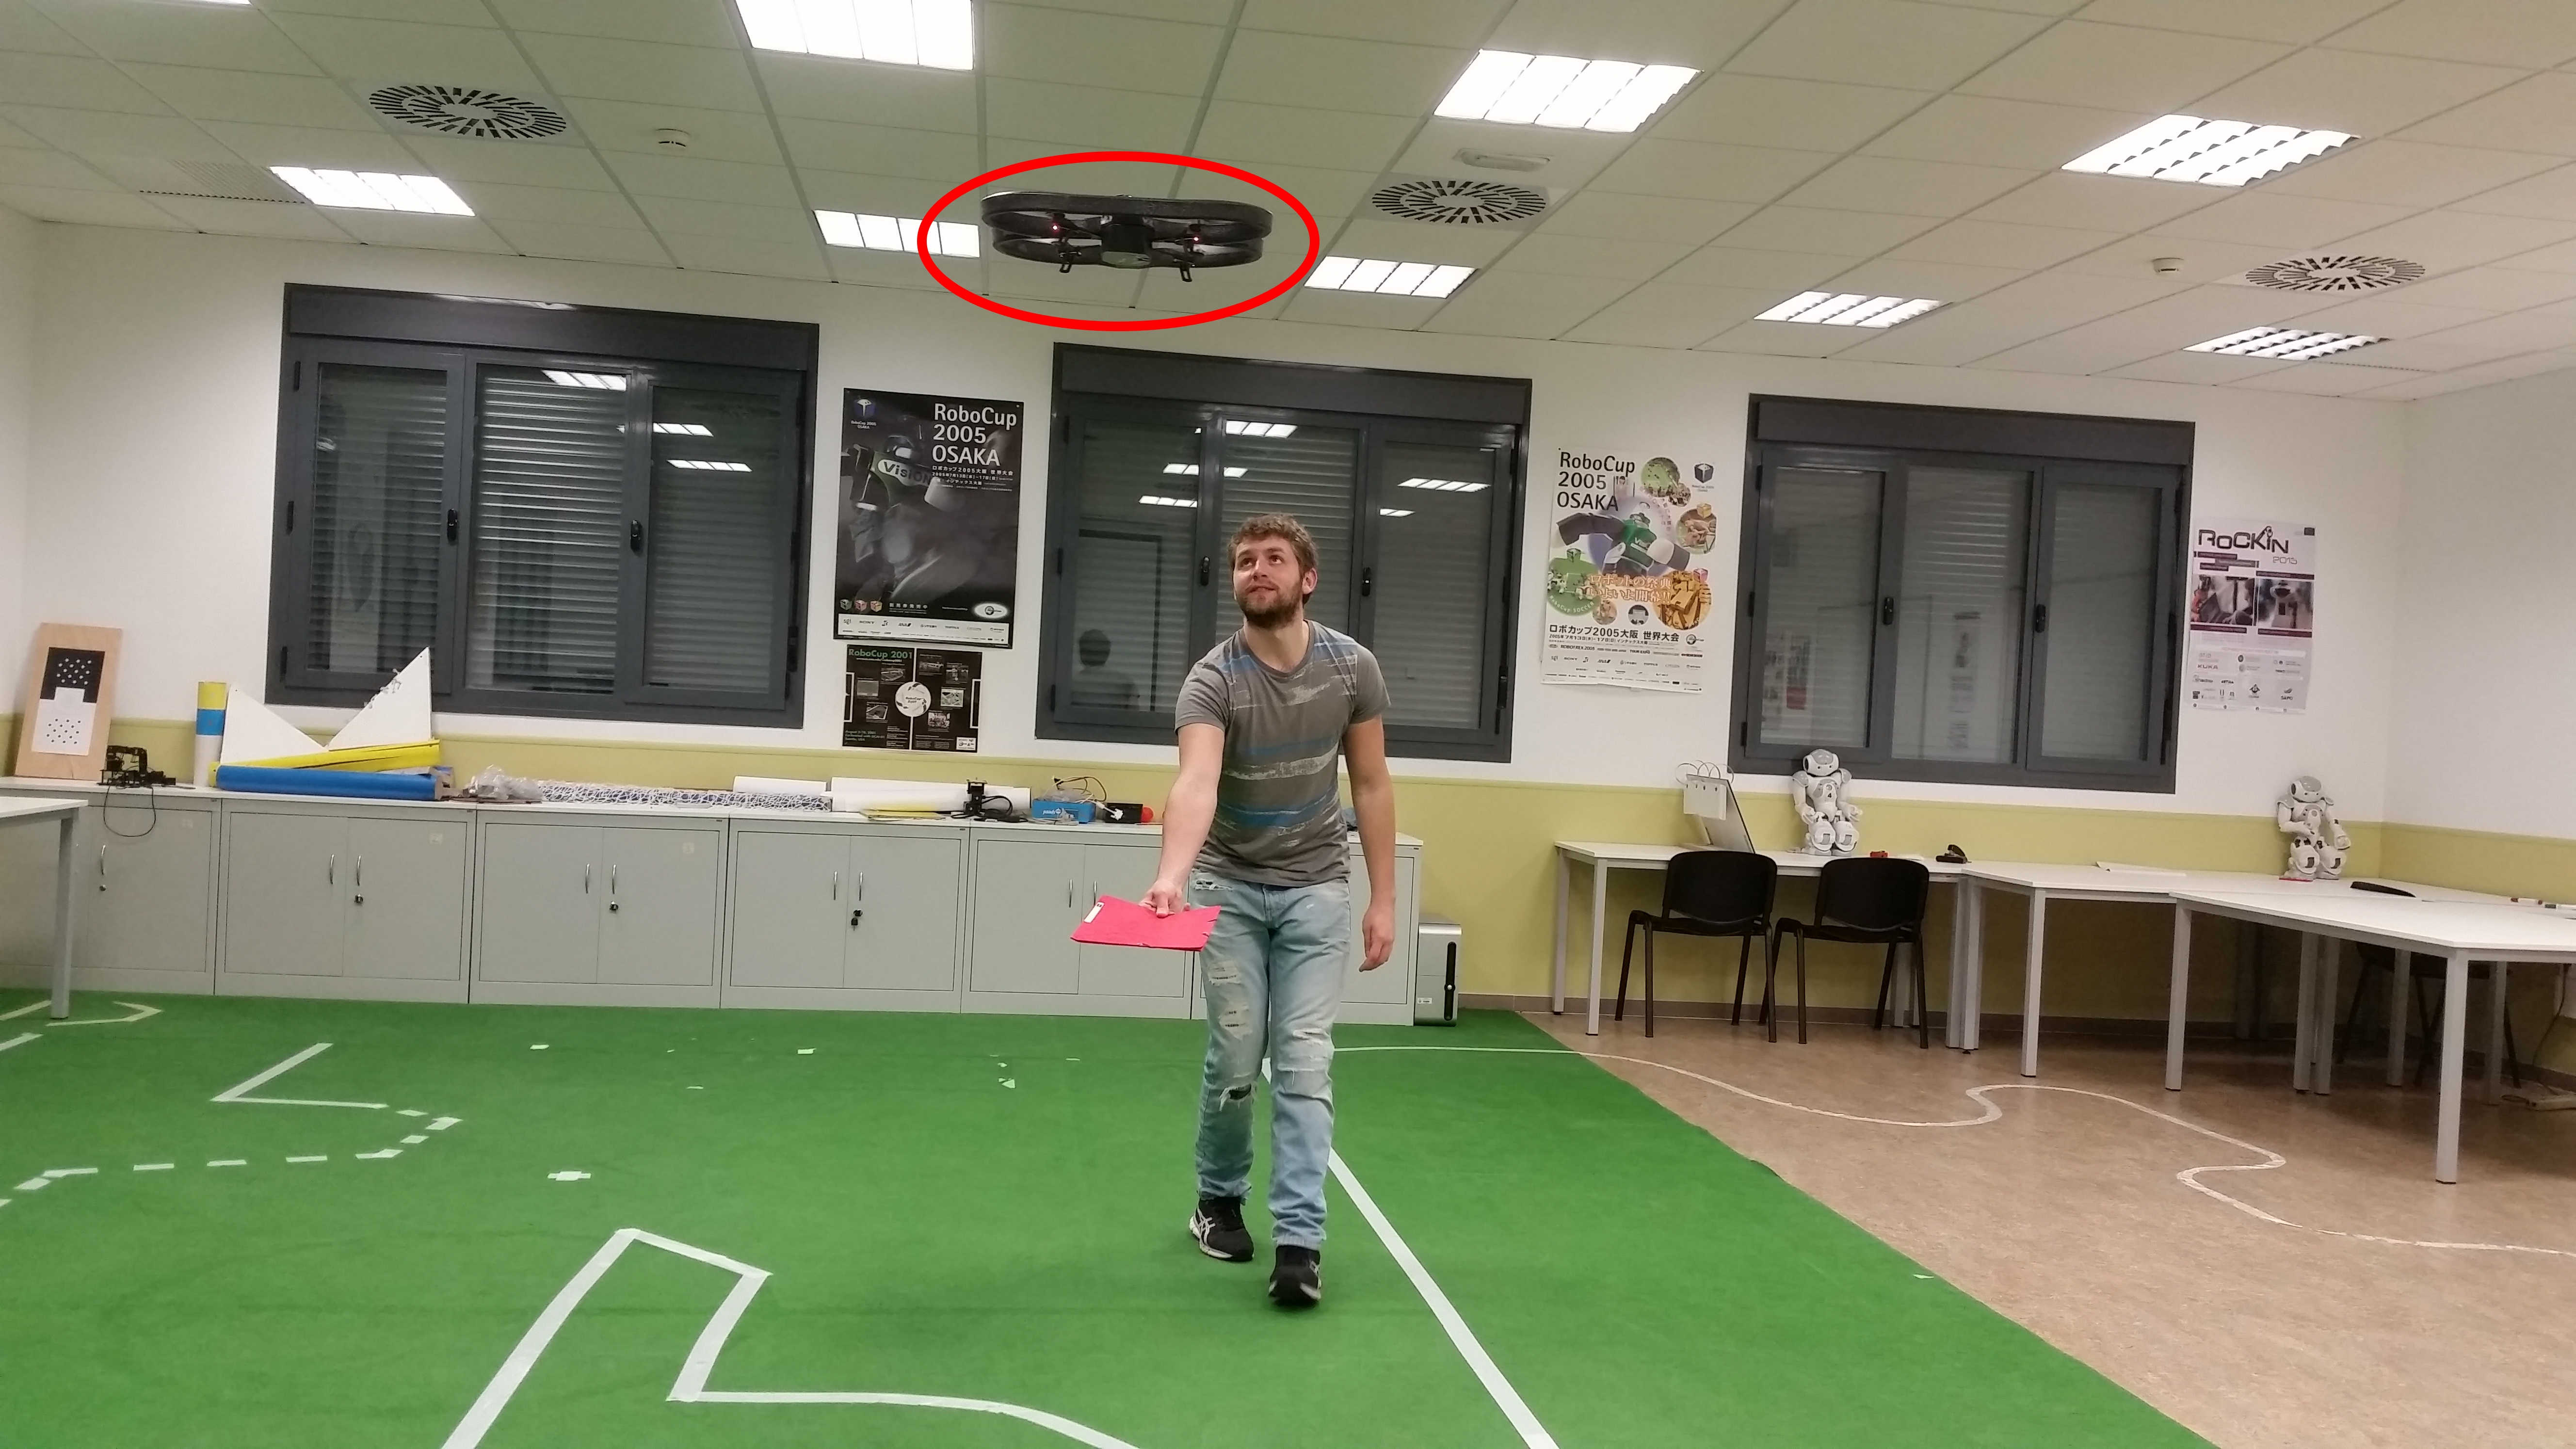
\includegraphics[height=3cm]{imgs/followingRed.jpg}
	\end{figure}
\end{minipage}
\end{center}

\end{hslide}

%%--------------------------------------------------------------


\end{document}

